% This is text associated with the open textbook "Open Electromagnetics"
% See immediately below for author, date
% This work is licensed under the Creative Commons Attribution-ShareAlike 4.0 International License. (CC BY SA 4.0) 
% To view a copy of the license, visit http://creativecommons.org/licenses/by-sa/4.0/

%ORB TITLE The Biot-Savart Law
%ORB AUTHOR 0        # S.W. Ellingson, Virginia Tech (ellingson@vt.edu)
%ORB DATE 20191128   # yyyymmdd
%ORB ABSTRACT 

\label{m0066_Biot-Savart} % <-- Must match name of this file and module directory name.  Don't mess with this!
\index{Biot-Savart law|(}

The Biot-Savart law (BSL) provides a method to calculate the magnetic field due to any distribution of steady (DC) current.
In magnetostatics, the general solution to this problem employs Ampere's law; 
\index{Ampere's law!magnetostatics}
i.e.,
%
\begin{equation}
\int_{\mathcal C} {\bf H} \cdot d{\bf l} = I_{encl} 
\end{equation}
%
in integral form or 
%
\begin{equation}
\nabla \times {\bf H} = {\bf J} 
\end{equation}
%
in differential form.
The integral form is relatively simple when the problem exhibits a high degree of symmetry, facilitating a simple description in a particular coordinate system.  
An example is the magnetic field due to a straight and infinitely-long current filament, which is easily determined by solving the integral equation in cylindrical coordinates.  
However, many problems of practical interest do not exhibit the necessary symmetry.
A commonly-encountered example is the magnetic field due to a single loop of current, which will be addressed in Example~\ref{m0066_exCircularLoopCurrent}.
For such problems, the differential form of Ampere's law is needed.

BSL is the solution to the differential form of Ampere's law for a differential-length current element, illustrated in Figure~\ref{m0066_fBSL}.
The current element is $I~d{\bf l}$, where $I$ is the magnitude of the current (SI base units of A) and $d{\bf l}$ is a differential-length vector indicating the direction of the current at the ``source point'' ${\bf r}'$.
The resulting contribution to the magnetic field intensity at the ``field point'' ${\bf r}$ is
%
\begin{equation}
\boxed{
d{\bf H}({\bf r}) = I~d{\bf l}~\frac{1}{4\pi R^2} \times \hat{\bf R}
}
\label{m0066_eBS}
\end{equation}
%
where 
%
\begin{equation}
{\bf R} = \hat{\bf R}R \triangleq {\bf r} - {\bf r}'
\end{equation}
%
In other words, ${\bf R}$ is the vector pointing from the source point to the field point, and $d{\bf H}$ at the field point is given by Equation~\ref{m0066_eBS}.
The magnetic field due to a current-carrying wire of any shape may be obtained by integrating over the length of the wire:
%
\begin{equation}
{\bf H}({\bf r}) = \int_{\mathcal{C}} d{\bf H}({\bf r}) = \frac{I}{4\pi} \int_{\mathcal{C}} \frac{d{\bf l}\times \hat{\bf R}}{R^2}
\label{m0066_eBSI} 
\end{equation}
%
\begin{figure}[b!] % <--- "[b]" for first figure in section *only*; delete for 2nd and subsequent figures
\begin{center}
\pdftooltip{{  % note double braces
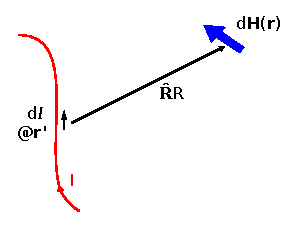
\includegraphics[width=2in]{modules/m0066_fBSL.eps} 
% https://commons.wikimedia.org/wiki/File:M0003_fBarMagnet.svg
}}{Vector labeled boldface capital R hat capital R points away from a wire in the presence of a magnetic field. The  wire with current I moving from bottom to top has a current differential d I at a source point small r prime which is roughly center. Thick directional arrow of magnetic field intensity, denoted small d boldface capital H of r, is perpendicular to the wire and the vector between the wire and itself.}
\end{center}
\centerline{\scriptsize 
\copyright~\hyperref[m0066_fBSL_Credit]{C.\ Wang} 
\href{https://creativecommons.org/licenses/by/4.0/}{CC BY-SA 4.0} 
} % \centerline 
\caption{
\label{m0066_fBSL}
Use of the Biot-Savart law to calculate the magnetic field due to a line current.
}
\end{figure}

In addition to obviating the need to solve a differential equation, BSL provides some useful insight into the behavior of magnetic fields.
In particular, Equation~\ref{m0066_eBS} indicates that magnetic fields follow the \emph{inverse square law}
\index{inverse square law}
-- that is, the magnitude of the magnetic field due to a differential current element decreases in proportion to the inverse square of distance ($R^{-2}$).
Also, Equation~\ref{m0066_eBS} indicates that the direction of the magnetic field due to a differential current element is perpendicular to both the direction of current flow $\hat{\bf l}$ and the vector $\hat{\bf R}$ pointing from the source point to field point. 
This observation is quite useful in anticipating the direction of magnetic field vectors in complex problems.
 
It may be helpful to note that BSL is analogous to Coulomb's law
\index{Coulomb's law}
for electric fields, which is a solution to the differential form of Gauss' law, $\nabla \cdot {\bf D} = \rho_v$.
\index{Gauss' law!electric field}
However, BSL applies only under magnetostatic conditions.  If the variation in currents or magnetic fields over time is significant, then the problem becomes significantly more complicated.  See ``Jefimenko's Equations'' 
\index{Jefimenko's equations}
in ``Additional Reading'' for more information.

%%%%%%%%%%%%%%%%%%%%%%%%%%%%%%%%%%%%%%%%%%%%%%%%%%%%%%%%%%%%%%%%%
%ORB EXAMPLE
~\\ \begin{example} 
\label{m0066_exCircularLoopCurrent}
\begin{mdframed}[backgroundcolor=brown!20,linecolor=brown!20]\raggedright
Magnetic field along the axis of a circular loop of current.
\\~\\
Consider a ring of radius $a$ in the $z=0$ plane, centered on the origin, as shown in Figure~\ref{m0066_fCCL}.
As indicated in the figure, the current $I$ flows in the $\hat{\bf \phi}$ direction.
Find the magnetic field intensity along the $z$ axis.

{\bf Solution.}
The source current position is given in cylindrical coordinates as
%
\begin{equation}
{\bf r}' = \hat{\bf \rho}a  
\end{equation}
%
The position of a field point along the $z$ axis is
%
\begin{equation}
{\bf r} = \hat{\bf z}z  
\end{equation}
%
Thus,
%
\begin{equation}
\hat{\bf R}R \triangleq {\bf r}-{\bf r}' = -\hat{\bf \rho}a + \hat{\bf z}z  
\end{equation}
%
and
%
\begin{equation}
R \triangleq \left|{\bf r}-{\bf r}'\right| = \sqrt{a^2+z^2} 
\end{equation}

Equation~\ref{m0066_eBS} becomes:
%
\begin{flalign}
d{\bf H}(\hat{\bf z}z) &= \frac{I~\hat{\bf\phi}~ad\phi}{4\pi \left[a^2+z^2\right]} \times \frac{\hat{\bf z}z-\hat{\bf \rho}a}{\sqrt{a^2+z^2}} \nonumber \\
                       &= \frac{Ia}{4\pi} ~ \frac{ \hat{\bf z}a-\hat{\bf \rho}z }{\left[a^2+z^2\right]^{3/2}} ~ d\phi
\end{flalign}
%
Now integrating over the current:
%
\begin{flalign}
&{\bf H}(\hat{\bf z}z) = \int_{0}^{2\pi} { \frac{Ia}{4\pi} ~ \frac{ \hat{\bf z}a - \hat{\bf \rho}z }{\left[a^2+z^2\right]^{3/2}} ~ d\phi  }& 
\end{flalign}
\begin{flalign}
&= \frac{Ia}{4\pi \left[a^2+z^2\right]^{3/2}} \int_{0}^{2\pi} { \left( \hat{\bf z}a - \hat{\bf \rho}z \right) ~ d\phi  }&  
\end{flalign}
\begin{flalign}
&= \frac{Ia}{4\pi \left[a^2+z^2\right]^{3/2}} \left( \hat{\bf z}a \int_{0}^{2\pi} { d\phi  } -z \int_{0}^{2\pi} { \hat{\bf \rho} ~ d\phi  }\right)&
\end{flalign}
%
The second integral is equal to zero.
To see this, note that the integral is simply summing values of $\hat{\bf\rho}$ for all possible values of $\phi$.  
Since $\hat{\bf\rho}(\phi+\pi)=-\hat{\bf\rho}(\phi)$, the integrand for any given value of $\phi$ is equal and opposite the integrand $\pi$ radians later.
(This is one example of a \emph{symmetry} argument.) 

The first integral in the previous equation is equal to $2\pi$.
Thus, we obtain
%
\begin{equation}
{\bf H}(\hat{\bf z}z) = \hat{\bf z}\frac{I a^2}{2\left[a^2+z^2\right]^{3/2}} 
\end{equation}
%
Note that the result is consistent with the associated ``right hand rule'' 
\index{right hand rule!magnetostatics}
of magnetostatics:  That is, the direction of the magnetic field is in the direction of the curled fingers of the right hand when the thumb of the right hand is aligned with the location and direction of current. 
It is a good exercise to confirm that this result is also dimensionally correct.
\end{mdframed}
%
\begin{figure}
\begin{center}
\pdftooltip{{  % note double braces

\includegraphics[width=2in]{modules/m0066_fCCL.eps} 
% https://commons.wikimedia.org/wiki/File:M0104_fRing.svg originally, but I added the "I" and arrow indicating current direction
}}{Cartesian coordinate system shown with x, y, and z axes. A red ring indicating current lies in the x and y plane, with its center at the origin, and with an arrow indicating counterclockwise current flow as viewed from above the plane. The radius of the circle is labeled bold rho hat * a. From the point at which the radius reaches the outside of the circle extends a ray labeled bold r - bold r', pointing to an arbitrary field point along the z-axis. }
\end{center}
\centerline{\scriptsize 
\copyright~\hyperref[m0066_fCCL_Credit]{K.\ Kikkeri} 
\href{https://creativecommons.org/licenses/by-sa/4.0/}{CC BY~SA 4.0} 
(modified)
} 
\caption{
\label{m0066_fCCL}
Calculation of the magnetic field along the $z$ axis due to a circular loop of current centered in the $z=0$ plane.
}
\end{figure}
%
\end{example}
%%%%%%%%%%%%%%%%%%%%%%%%%%%%%%%%%%%%%%%%%%%%%%%%%%%%%%%%%%%%%%%%%

Equation~\ref{m0066_eBS} extends straightforwardly to other distributions of current. 
For example, the magnetic field due to surface current ${\bf J}_s$ (SI base units of A/m) can be calculated using Equation~\ref{m0066_eBS} with $I~d{\bf l}$ replaced by 
$${\bf J}_s~ds$$
where $ds$ is the differential element of surface area. 
This can be confirmed by dimensional analysis: $I~d{\bf l}$ has SI base units of A$\cdot$m, as does ${\bf J}_S~ds$.
Similarly, the magnetic field due to volume current ${\bf J}$ (SI base units of A/m$^2$) can be calculated using Equation~\ref{m0066_eBS} with $I~d{\bf l}$ replaced by 
$${\bf J}~dv$$ 
where $dv$ is the differential element of volume.
For a single particle with charge $q$ (SI base units of C) and velocity ${\bf v}$ (SI base units of m/s), the relevant quantity is
$$ q{\bf v} $$
since C$\cdot$m/s $=$ (C/s)$\cdot$m = A$\cdot$m. 
In all of these cases, Equation~\ref{m0066_eBS} applies with the appropriate replacement for $I~d{\bf l}$.

Note that the quantities $q{\bf v}$, $I~d{\bf l}$, ${\bf J}_S~ds$, and ${\bf J}~dv$, all having the same units of A$\cdot$m, seem to be referring to the same physical quantity.
This physical quantity is known as \emph{current moment}.
\index{current moment} 
Thus, the ``input'' to BSL can be interpreted as current moment, regardless of whether the current of interest is distributed as a line current, a surface current, a volumetric current, or simply as moving charged particles.
See ``Additional Reading'' at the end of this section for additional information on the concept of ``moment'' in classical physics.

%%%%%%%%%%%%%%%%%%%%%

{\bf Additional Reading:}
\begin{itemize}
\item ``\href{https://wikipedia.org/wiki/Biot-Savart_law}{Biot-Savart Law}'' on Wikipedia.
\item ``\href{https://wikipedia.org/wiki/Jefimenko's_equations}{Jefimenko's Equations}'' on Wikipedia.
\item ``\href{https://en.wikipedia.org/wiki/Moment_(physics)}{Moment (physics)}'' on Wikipedia.

\end{itemize}

\index{Biot-Savart law|)}
